% Chapter Template

\chapter{Image processing} % Main chapter title

\label{Chapitre 4.1} % Change X to a consecutive number; for referencing this chapter elsewhere, use \ref{ChapterX}

\lhead{ \emph{Traitement des images}} % Change X to a consecutive number; this is for the header on each page - perhaps a shortened title

%----------------------------------------------------------------------------------------
%	SECTION 1
%----------------------------------------------------------------------------------------
Le but de ce chapitre est de vous parler un peu de l'amélioration du traitement d'image pour obtenir de meilleurs résultats.

\section{Process image code}


\begin{lstlisting}[frame=single,style=Python]  % Start your code-block

def process_image(im, border_size=8, im_size=50):
    """ Remove borders and resize """

    sx, sy = im.shape;

    # noise removal
    im = median(im, disk(2))

    # binarization
    thresh = threshold_otsu(im)
    im = im > thresh
	  
    # erosion
    im = erosion(im, disk(1))

    im = im[ sx/8:-sx/8, sy/8:-sy/8]

    im = resize(im , (im_size, im_size))

    # Si la case est presque blanche
    if (np.mean(im) >= 0.9) :
	im[:,:] = 1.0
    elif (np.mean(im) <= 0.2) :
	im[:,:] = 1.0
    return im
\end{lstlisting}


\pagebreak
Ce qui nous donne les résultats suivant : \\


\textbf{Sans traitement d'image :}
\begin{center} 
\hspace{15cm}
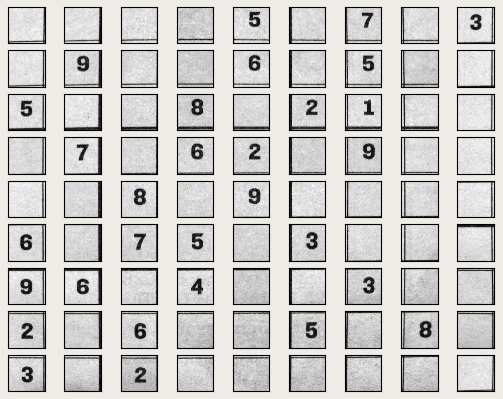
\includegraphics[width=12cm]{Avant_Processing.png}
\end{center}
\vspace{0.5cm} 

\textbf{Avec traitement d'image :}
\begin{center} 
\hspace{15cm}
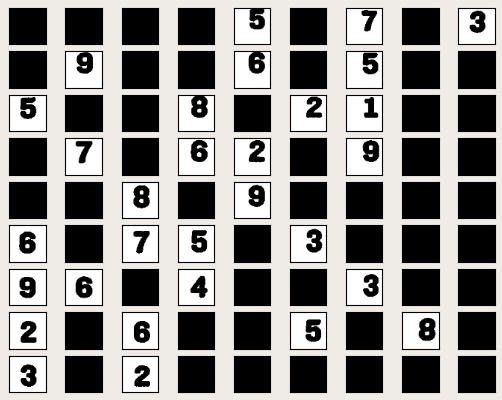
\includegraphics[width=12cm]{Apres_Processing.png}
\end{center}
\vspace{0.5cm} 

Ce qui rend nos cases considérablement plus lisible. Par contre, les cases noires devraient être blanches. Nous n'avons pas compris (même en forcant un valeur soit 0 où 1).

